\documentclass{article}
\usepackage{amsmath}
\usepackage{graphicx}
\usepackage{caption}
\usepackage{subcaption}
\usepackage{hyperref}
\usepackage{glossaries}
\usepackage{acronym}
\usepackage{nomencl}
\usepackage{pdfpages}
\usepackage{datetime}
\usepackage{lscape}
\usepackage{changepage}
\makeglossaries
\newacronym{gpu}{GPU}{graphics processing unit}
\newglossaryentry{latex}{name=LaTeX, description={A typesetting system}}

\begin{document}
\section{Acronyms}
The \gls{gpu} is fast. A \acrfull{gpu} again, \acrshort{gpu}, \acrlong{gpu}, \Gls{latex}, \glspl{gpu}.

\begin{acronym}
\acro{CPU}{Central Processing Unit}
\acro{RAM}{Random Access Memory}
\end{acronym}
We use a \ac{CPU} and \ac{RAM}; again the \ac{CPU}. Plural \acp{CPU}.

\section{Figures}
\begin{figure}[ht]
  \centering
  \captionsetup[subfigure]{justification=centering}
  \begin{subfigure}{0.3\textwidth}
    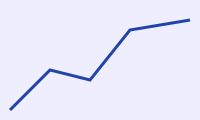
\includegraphics[width=\textwidth]{plot.svg}
    \caption{One}\label{fig:one}
  \end{subfigure}
  \begin{subfigure}{0.3\textwidth}
    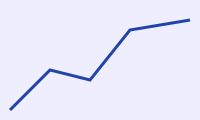
\includegraphics[width=\textwidth]{diagram.svg}
    \caption{Two}\label{fig:two}
  \end{subfigure}
  \caption{Two subfigures.}\label{fig:both}
\end{figure}

\begin{adjustwidth}{1cm}{1cm}
Indented both sides.
\end{adjustwidth}

Printed on \currenttime, \today.

\printglossaries
\printnomenclature
\end{document}
